\documentclass[12pt,a4paper,bibliography=totocnumbered,listof=totocnumbered]{scrartcl}
\usepackage[ngerman]{babel}
\usepackage[utf8]{inputenc}
\usepackage{amsmath}
\usepackage{amsfonts}
\usepackage{amssymb}
\usepackage{graphicx}
\usepackage{fancyhdr}
\usepackage{tabularx}
\usepackage{geometry}
\usepackage{setspace}
\usepackage[right]{eurosym}
\usepackage[printonlyused]{acronym}
\usepackage{subfig}
\usepackage{floatflt}
\usepackage[usenames,dvipsnames]{color}
\usepackage{colortbl}
\usepackage{paralist}
\usepackage{array}
\usepackage{titlesec}
\usepackage{parskip}
\usepackage[right]{eurosym}
\usepackage{picins}
\usepackage[subfigure,titles]{tocloft}
\usepackage[pdfpagelabels=true]{hyperref}
\usepackage{bchart}



\usepackage{listings}
\lstset{basicstyle=\footnotesize, captionpos=b, breaklines=true, showstringspaces=false, tabsize=2, frame=lines, numbers=left, numberstyle=\tiny, xleftmargin=2em, framexleftmargin=2em}
\makeatletter
\def\l@lstlisting#1#2{\@dottedtocline{1}{0em}{1em}{\hspace{1,5em} Lst. #1}{#2}}
\makeatother

\geometry{a4paper, top=27mm, left=20mm, right=20mm, bottom=35mm, headsep=10mm, footskip=12mm}


\hypersetup{unicode=false, pdftoolbar=true, pdfmenubar=true, pdffitwindow=false, pdfstartview={FitH},
	pdftitle={Wahlpflichtfach: Implementierung von Brettspielen am Beispiel ReversiXT},
	pdfauthor={Gruppe 10},
	pdfsubject={Projektbericht},
	pdfcreator={\LaTeX\ with package \flqq hyperref\frqq},
	pdfproducer={pdfTeX \the\pdftexversion.\pdftexrevision},
	pdfkeywords={Projektbericht, ReversiXT},
	pdfnewwindow=true,
	colorlinks=true,linkcolor=black,citecolor=black,filecolor=magenta,urlcolor=black}
\pdfinfo{/CreationDate (D:20151500000000)}

\begin{document}

\titlespacing{\section}{0pt}{12pt plus 4pt minus 2pt}{-6pt plus 2pt minus 2pt}

% Kopf- und Fusszeile
\renewcommand{\sectionmark}[1]{\markright{#1}}
\renewcommand{\leftmark}{\rightmark}
\pagestyle{fancy}
\lhead{}
\chead{}
\rhead{\thesection\space\contentsname}
\lfoot{Implementierung von Brettspielen am Beispiel ReversiXT -- SS 2015}
\cfoot{}
\rfoot{\ \linebreak Seite \thepage}
\renewcommand{\headrulewidth}{0.4pt}
\renewcommand{\footrulewidth}{0.4pt}

% Vorspann
\renewcommand{\thesection}{\Roman{section}}
\renewcommand{\theHsection}{\Roman{section}}
\pagenumbering{Roman}

\newcommand{\folgen}[1]{
\ensuremath
#1
}

\newcommand{\MyTitlepage}[5][\empty]{
\thispagestyle{empty}
\begin{center}
	
\includegraphics[scale=1]{pics/oth-logo.png}\\
	\vspace*{2cm}
	\Large
	\textbf{Fakultät}\\
	\textbf{Informatik und Mathematik}\\
	\vspace*{2cm}
	\Huge
	\textbf{Projektbericht}\\
	\vspace*{0.5cm}
	\large
	zum Wahlpflichtfach\\
	\vspace*{1cm}
	\textbf{Implementierung von Brettspielen am Beispiel ReversiXT}\\
	\vspace*{1cm}
	\includegraphics[height=6cm]{#1}
	\vfill
	\normalsize
	%\newcolumntype{x}[1]{>{\raggedleft\arraybackslash\hspace{0pt}}p{#1}}
	\begin{tabular}{rl}%{6cm}p{7.5cm}}
	    \rule{0mm}{5ex}\textbf{Gruppe:} & #2 \\
		\rule{0mm}{5ex}\textbf{Autor:} & \hspace*{-0.5em}\begin{tabular}[t]{l}#3\end{tabular} \\ 
		\rule{0mm}{5ex}\textbf{Leiter:} & Prof. Dr. rer. nat. Carsten Kern \\ 
		\rule{0mm}{5ex}\textbf{Abgabedatum:} & #4 \\ 
	\end{tabular} 
\end{center}
\pagebreak
}
% ----------------------------------------------------------------------------------------------------------
% Titelseite
% ----------------------------------------------------------------------------------------------------------
\MyTitlepage[pics/gamefield02]{10}{Florian Fußeder\\Sebastian Sidortschuck\\Peter Repukat}{05.07.2015} % FIXME optional: Gruppenlogo als PNG, Pflichtfelder: Gruppe, Authoren durch "\\" getrennt und Abgabedatum eingeben

\setcounter{page}{1} 
% ----------------------------------------------------------------------------------------------------------
% Inhaltsverzeichnis
% ----------------------------------------------------------------------------------------------------------
\tableofcontents
\pagebreak


% ----------------------------------------------------------------------------------------------------------
% Inhalt
% ----------------------------------------------------------------------------------------------------------
% Abstände Überschrift
\titlespacing{\section}{0pt}{12pt plus 4pt minus 2pt}{-6pt plus 2pt minus 2pt}
\titlespacing{\subsection}{0pt}{12pt plus 4pt minus 2pt}{-6pt plus 2pt minus 2pt}
\titlespacing{\subsubsection}{0pt}{12pt plus 4pt minus 2pt}{-6pt plus 2pt minus 2pt}

% Kopfzeile
\renewcommand{\sectionmark}[1]{\markright{#1}}
\renewcommand{\subsectionmark}[1]{}
\renewcommand{\subsubsectionmark}[1]{}
\lhead{Kapitel \thesection}
\rhead{\rightmark}

\onehalfspacing
\renewcommand{\thesection}{\arabic{section}}
\renewcommand{\theHsection}{\arabic{section}}
\setcounter{section}{0}
\pagenumbering{arabic}
\setcounter{page}{1}

% ----------------------------------------------------------------------------------------------------------
% Einleitung
% ----------------------------------------------------------------------------------------------------------
\section{Allgemeine Informationen}
\begin{itemize}
\item Programmiersprache: C++11
\item IDE Windows: Visual Studio 2013/2015
\item Compiler Linux: GCC g++
\end{itemize}

\section{Core-System}
In diesem Abschnitt wird des Grundsystem für das Einlesen der Map und dem Setzen von Spielsteinen betrachtet

\subsection{Einlesen}
Zu Beginn des Spieles wird von unserem Client die Map eingelesen.
Gespeichert wird das Spielfeld als ein 2-dimensionaler Vector von structs, nach dem im nachfolgenden Quellcode angegebenen Format:


\vspace{1em}
\begin{lstlisting}[caption=Feld, label=lst:Feld.h]
struct Feld{

		enum Art : char
		{
			Hole = '-',
			Empty = '0',
			Choice = 'c',
			Inversion = 'i',
			Bonus = 'b',
			Expansion = 'x'
		};


		
		char art;														//Identifikationszeichen
		bool playerField;												//Spieleridentifikation true wenn Spieler drauf liegt
		std::unordered_map<short, turnPos> Transition;
		Feld() :art(Art::Hole), playerField(false), Transition(){}
		Feld(char c) :art(c), playerField(false), Transition(){}
	};
\end{lstlisting}
\pagebreak

\subsection{Finden von Ecken}
Für die später beschriebene Bewertungsfunktion ist es notwendig die Ecken des Feldes zu finden, da diese im Spielverlauf eine besondere Bedeutung haben.
Um diese zu finden wird beim Einlesen des Spielfeldes jede Position daraufhin überprüft,  beginnend bei den 4 Grundrichtungen(0,2,4,6), ob es drei aufeinanderfolgende Positionen gibt, die entweder außerhalb des Spielfeldes sind, oder mit '-' belegt sind. Falls dies der Fall ist, wird in dem Feld ein bool gesetzt der dies kennzeichnet.

\subsection{Berechnung möglicher Spielzüge}
Für einen möglichen Zug muss mindestens ein Stein eines Gegners übernommen werden. Dafür müssen Folgende Voraussetzungen erfüllt sein:
\begin{itemize}
	\item Ein Stein muss auf ein leeres Feld gelegt werden.
	\item Es müssen sich gegnerische Spielsteine zwischen einem bereits gesetzten und dem zu setzenden Spielstein befinden.
	\item Das einschließen gilt immer nur bist zum nächsten eigenen Spielstein.
	\item Bei den einschließenden Steinen darf es sich nicht um den selben Stein handeln (es gelten keine Zyklen)
\end{itemize}


\subsection{Algorithmus}
Die Dateien Turns.cpp und Turns.h ermitteln die möglichen Züge, hier werden die Koordinaten und die Richtungen in die dann umgefärbt werden muss ermittelt.
Der Algorithmus arbeitet wie folgt:
\begin{itemize}
\item In dem std::vector startpos sind die Positionen aller Spielsteine eines Spieler vermerkt.
\item Nun wird von jedem Stein in die möglichen 8 Richtungen (0, 1, 2, 3, 4, 5, 6, 7) gelaufen
\item Falls das Feld eine Transition besitzt wird dieser gefolgt
\item Anderenfalls wird der Richtung gefolgt bis einer der Folgenden Fälle eintritt:
\begin{itemize}
\item Man trifft auf ein '-' oder das Ende der Map
\begin{itemize}
\item Es konnte kein leeres Feld gefunden werden $\Rightarrow$ kein Gültiger Zug
\end{itemize}
\item Man trifft auf einen der eigenen Spielsteine
\begin{itemize}
\item Es können keine gegnerischen Steine eingeschlossen werden $\Rightarrow$ kein Gültiger Zug
\end{itemize}
\item Man trifft auf ein leeres Feld
\begin{itemize}
\item Der Abstand zur Startposition beträgt 1 $\Rightarrow$ kein Gültiger Zug
\item Der Abstand zur Startposition ist $\ge$ 1 $\Rightarrow$ Gültiger Zug
\end{itemize}
\end{itemize}
\end{itemize}



Ist ein gültiger Zug gefunden, wird dessen Position und die Richtung aus der man den Zug ermittelt hat, in einer unorderd\_map \textless Richtung, Position\textgreater abgelegt. So kann man zum setzen eines Steines einfach den abgespeicherten Richtungen folgen und muss nicht nochmal in alle Richtungen überprüfen.


\pagebreak
\subsection{Ausführen der Spielzüge}
Zur Ausführung der Spielzüge wird an die Funktion ExecTurn ein gültiger Spielzug übergeben mit X, Y Koordinate der Startposition und einem std::vector in dem mögliche Richtungen gespeichert werden.
Die Funktion arbeitet wie folgt:
\begin{itemize}
\item Das Feld auf welches der neue Stein gesetzt wird, wird auf Spezialeigenschaften überprüft und der neue Stein gesetzt
\item Nun werden in die erste mögliche Richtung Koordinaten der zu ersetzenden Felder in einem std::vector gespeichert
\item Wenn auf ein Feld des ausführenden Spielers getroffen wird, gilt die jeweilige Richtung als abgeschlossen und die nächste wird behandelt
\item Wenn auf eine Transition getroffen wird, wird die Eingangsrichtung überprüft, stimmt diese mit der Zugrichtung überein wird vom Ausgangsfeld der Transition in ihrer Ausgangsrichtung weiter ersetzt
\item Danach werden vermerkten Koordinaten der zu ersetzenden Felder durch Felder des ausführenden Spielers ersetzt
\end{itemize}
Nun erfolgt die Behandlung der Spezialfelder
\begin{itemize}
\item Falls auf ein Bonusfeld gesetzt wurde, wird dem Spieler der gewählte Bonus, Bombe oder Überschreibstein gutgeschrieben
\item Falls auf ein Inversionsfeld gesetzt wurde, wird die Map abgelaufen und die Spielersteine um 1 erhöht, im Falle einer zu großen Zahl wird diese auf den ersten Spieler gesetzt
\item Falls auf ein Choicefeld gesetzt wurde
\begin{itemize}
\item Koordinaten der Steine des gewählten Tauschpartners in einem std::vector gespeichert
\item Eigene Steine durch die des Tauschpartners ersetzt
\item Die gespeicherten Steine des gewählten Tauschpartners werden nun durch eigene Steine ersetzt 
\end{itemize}
\item Zu guter Letzt werden die gültigen Züge gelöscht, so wie die Startpositionen für die Berechnung der gültigen Spielzüge neu errechnet.
\end{itemize}
Da davon ausgegangen wird, dass die übergebenen Züge gültig sind, erfolgt keine Fehlerbehandlung.
\subsection{Ausführen der Spielzüge im Falle eines Überschreibzuges}
Im Fall eines Überschreibzuges, wird der Funktion ExecTurn keine Richtung mitgegeben.
In einem solchen Fall funktioniert die Zugausführung wie die, der normalen Züge,
allerdings wird in alle 8 Richtungen geprüft (die zu ersetzenden Steine werden in 8 std::vector vorgemerkt) und für den Fall das eine Richtung nicht möglich sein sollte, der std::vector mit vorgemerkten Steinen zurückgesetzt und somit beim schlussendlichen Umfärben ignoriert.
\pagebreak

% ----------------------------------------------------------------------------------------------------------
% Bewertung von Spielzuständen
% ----------------------------------------------------------------------------------------------------------
\section{Bewertung von Spielzuständen}
Um Entscheidung über den nächsten Zug zu machen muss es ermöglicht werden jeden Spielzustand bewerten zu können.
In diesem Kapitel werden nun die verwendeten Funktionen vorgestellt.

\subsection{Bewertung anhand von Wertigkeiten unterschiedlicher Felder}
In diesem Verfahren ist der Grundgedanke, dass jedes Feld eine unterschiedliche Wertigkeit besitzt.
Es wird hierfür vorausgesetzt, dass die möglichen Züge aller Spieler immer aktuell gehalten werden.
\vspace{1em}
Der Algorithmus läuft nun über alle möglichen Spielzüge und addiert die daraus folgenden Spielzustände anhand der folgenden Tabelle. 
\vspace{1em}

\begin{table}[!h]
	\centering
	\begin{tabular}{|l|l|l|}
		\hline
		\textbf{Name} & \textbf{Wertigkeit}\\
		\hline
		 Möglicher Spielzug & 10\\
		\hline
		Besetztes Feld  &  10\\
		\hline
		Ecke & 300\\
		\hline
		Neben Ecke & -100\\
		\hline
		 Choicefeld & 350\\
		\hline
		Neben Choicefeld & -350\\
		\hline
		 Bonusfeld & 150\\
		\hline
		 Neben Bonus & -30\\
		\hline
		 Neben Inversion & -10\\
		\hline
	\end{tabular}
	\caption{Wertigkeitentabelle}
	\label{tab:Wertigkeit}
\end{table}

Dies wird für jeden Spieler ausgeführt. Im Anschluss wird der Zug ausgeführt, der zum einen das beste Verhältnis von der eigenen Veränderung zur Summe der Veränderung aller Gegenspieler bietet.


\pagebreak

\subsection{Idee: Verringerung der Außenflächen}
In diesem Verfahren wird versucht die Anzahl der Steine die außen liegen (\^= Nachbarn sind '0') zu verringern.
Das Ziel des Verfahrens ist es, dem Gegner möglichst wenig Zugmöglichkeiten offen zu legen. \\
Vorteile: 

\begin{itemize}
	\item Einfache Umsetzung
	\item Gibt einen Mobilitätsvorteil
	\item Gegner wird zu schlechten Zügen gezwungen
\end{itemize}

Nachteile: 

\begin{itemize}
	\item Aufwand(jedes Nachbarfeld von möglichen Zügen muss überprüft werden) \\
	=\textgreater  Lösung: Algorithmus nur auf gute Ergebnisse von anderen Verfahren anwenden
	\item Kann zu geringer Punktezahl während mancher Situationen führen
\end{itemize}

\pagebreak
\subsection{Paranoid Algorithmus}
Da der Algorithmus aufgrund der Vorlesung als bekannt angenommen wird, werden hier nur einige Besonderheiten unserer Implementierung erwähnt.
Da wir die Vorteile von foreach-Schleifen nutzen wollten ist der Algorithmus in 2 Teile unterteilt. Der erste Teil läuft mit einer Zählervariable über die Spielzüge die direkt Möglich sind, um nicht nur den Wert eines Zuges zu erkennen sondern auch die Position auf die der Stein gelegt wurde. Im zweiten Teil wird nicht betrachtet welcher Stein wohin gesetzt wurde sondern nur welchen Wert der Min- oder Max-Vergleich ergeben hat.
Des weiteren nutzen wir die Möglichkeit den zu ziehenden Spieler jeweils aus dem Spieler zu Beginn und der aktuellen  Tiefe zu errechnen
\pagebreak

\section{Bomben}
Um die beste Position für eine Bombe zu finden wird auf jedes mögliche Feld eine Bombe geworfen. Die Map wir aktualisiert und sogleich bewertet.

\begin{itemize}
\item Bombe werfen\\
Hier wird über die gesamte Map gelaufen und jedes Feld das nicht leer('-') ist eine Bombe geworfen
\item Ausführen der Bombe\\
Hier erfolgt das Ausführen mithilfe einer Queue. So wird das richtige Behandeln von Hindernissen und Transitionen gewährleistet. \\
Beispiel:
Bombenstärke 1\\
Das Feld ist nur von Spielsteinen umgeben und wird auf auf ein Feld mit den Koordinaten x, y geworfen. Die Koordinaten x,y wird mit der Bombenstärke zu einem struct zusammengefügt und in die Queue gelegt. Nun werden alle Felder um x,y herum mit (Bombenstärke -1) in die Queue geschoben. Dies passiert nun so oft, bist die Bombenstärke im struct 0 beträgt. Beträgt die Bombenstärke 0 so wird die Art des Feldes auf ein leeres Feld geändert. Sollten wir auf ein Feld mit einer Transition treffen legen wir dieses ein einen Vector ab und behandeln es später als wäre es eine Bombe mit der verbliebenen Stärke. Sogleich werden auch die Transitionen gelöscht damit keine Dauerschleife entsteht.
\item Bewerten der Map\\
Zuerst berechnen wir den Spieler, der von der Punktzahl vor uns ist. Nun suchen wir die Bombe, mit welcher wir den besten Wert für die Differenz aus unseren Punkten und den Punkten des Spielers vor uns erhalten. Somit wird gewährleistet das wir nicht unsere eigenen Steine zerstören, obwohl es nicht sein müsste und trotzdem dem Spieler vor uns größtmöglichen Schaden zufügen. Hier ein Ausschnitt:

\vspace{1em}
\begin{lstlisting}[caption=bombPos, label=lst:AlgorithmBase.cpp]
if (diffValue < myValue - EnemyNextValue){						
						diffValue = myValue - EnemyNextValue;

						if (EnemyBestValue >= EnemyNextValue){								
							EnemyBestValue = EnemyNextValue;								
							pos = ff::turnPos{ x, y };									
						}
\end{lstlisting}

\end{itemize}
\pagebreak
\section{Optimierung des Suchbaumes}
Um bessere Ergebnisse zu erreichen, wurde der Paranoid-Algorithmus um einige Funktionen erweitert.
\subsection{Auflistung der Optimierungen}
\begin{itemize}
\item Aspiration Window
\item Sortierung der Spielzüge
\item Alpha-Beta Pruning
\end{itemize}

\subsection{Verwendete Maps}
Um denn Speedup der verschiedenen Verfahren besser zu sehen wurden einige Testläufe gemacht.
Die Maps die hierfür verwendet wurden, sind in Abbildung 1 zu sehen.

\begin{figure}
\centering
\begin{minipage}[t]{1.8in}
{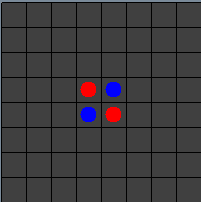
\includegraphics[width=1.8in]{pics/map_basic8x8}\caption*{Map: basic8x8}}
\end{minipage}
\begin{minipage}[t]{1.8in}
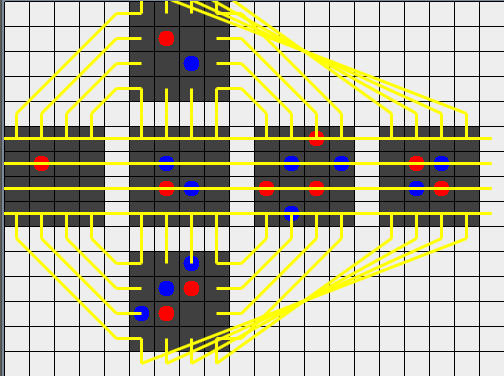
\includegraphics[width=1.8in]{pics/map_10_2p}\caption*{Map: 10\_2p}
\end{minipage}
\begin{minipage}[t]{1.8in}
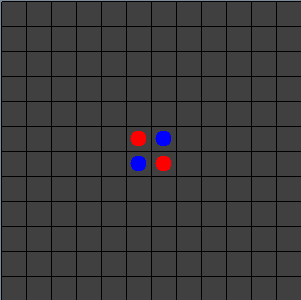
\includegraphics[width=1.8in]{pics/map_12x12}\caption*{Map: 12x12}
\end{minipage}
\caption{Verwendete Maps}
\end{figure}
\pagebreak
\subsection{Performance-Messung}
Messung der durchschnittlichen Zeit, die für Tiefe 5 auf der Map 12x12 benötigt wurden:

\begin{bchart}[max = 105]
\bcbar[label=Alles aktiviert,color=yellow]{2.213}
\bcbar[label=Ohne Sortieren,color=red]{2.377}
\bcbar[label=Ohne Alpha-Beta-Pruning und sortieren,color=green]{104.222}
\end{bchart}

Messung der durchschnittlichen Tiefe die innerhalb von 3 Sekunden erreicht werden konnte:
\begin{itemize}
\item Gelb = Alles aktiviert
\item Rot = Ohne Aspiration Window
\item Blau = Ohne Alpha-Beta-Pruning und ohne Sortieren
\item Grün = Ohne Optimierungen
\end{itemize}

\begin{bchart}[max = 11]
\bcbar[label= basic8x8,color=yellow]{9.926}
\bcbar[label= basic8x8,color=red]{10.444}
\bcbar[label= basic8x8,color=blue]{5.536}
\bcbar[label= basic8x8,color=green]{6.786}
\bigskip
\bcbar[label= 10\_2p,color=yellow]{7.914}
\bcbar[label= 10\_2p,color=red]{7.143}
\bcbar[label= 10\_2p,color=blue]{5.615}
\bcbar[label= 10\_2p,color=green]{4.971}
\bigskip
\bcbar[label= 12x12,color=yellow]{6.343}
\bcbar[label= 12x12,color=red]{6.397}
\bcbar[label= 12x12,color=blue]{4.611}
\bcbar[label= 12x12,color=green]{4.176}

\end{bchart}

\pagebreak
Um die Leistung des Alpha-Beta-Prunings besser zu zeigen, hier ein Auszug der erreichten Tiefen auf der Map:  "basic\_8x8" mit Zeitlimit von 3 Sekunden.
 
Mit A-B-Pruning:	14	14	14	13	14	11	10	10	8	10	9	9	10	10 	10 	10 	8	8	6	8	7	8	8	8	9	13	17  \\
Ohne A-B-Pruning:	 8	8	7	7	6	6	6	6	5	5	5	5	5	5	5	5	5	5	5	5	4	4	4	5	5	5	6	8 \\

\subsection{Zusammenfassung}
\begin{itemize}
\item Alpha-Beta-Pruning: \\
Wie man den gesammelten Daten entnehmen kann, bringt das Alpha-Beta-Pruning den größten Speedup, mit dem Faktor 1,5, dieser ist über die verschiedenen Maps relativ konstant.\\
Beim Durchspielen der Map: 12x12 mit Tiefenlimit 5, ergab sich eine durchschnittliche Zeitersparnis von 102 Sekunden pro Zug.
\item Sortieren:\\
Das Sortieren brachte im ausgewählten Beispiel einen Speedup von 1,1. Jedoch ist dies Abhängig davon, ob die Züge per Zufall in einer ungünstigen Reihenfolge gefunden werden, da dann das Sortieren unnötig Zeit braucht.
\item Aspiration Window:\\
Aus unseren Daten ist ersichtlich, dass diese Optimierung in manchen Fällen auch die Leistung verringern kann,siehe Daten basic8x8(Speedup = 0,95), dies geschieht durch ein zu geringes Fenster, wodurch manche Tiefen mehrfach berechnet werden müssen. Jedoch führt das Aspiration Window häufig zu einem besseren Ergebnis, siehe Daten 10\_2p(Speedup = 1,1).
\item Gesamt:\\
Aus den bei uns gemessen Ergebnissen können wir ein durchschnittlichen Speedup für alle Optimierungen von 1,51 ausgehen.

\end{itemize}


\end{document}
